\documentclass[11pt,compress,t,notes=noshow, xcolor=table]{beamer}
\usepackage[]{graphicx}\usepackage[]{color}
% maxwidth is the original width if it is less than linewidth
% otherwise use linewidth (to make sure the graphics do not exceed the margin)
\makeatletter
\def\maxwidth{ %
  \ifdim\Gin@nat@width>\linewidth
    \linewidth
  \else
    \Gin@nat@width
  \fi
}
\makeatother

\newcommand{\citebutton}[2]{%
\beamergotobutton{\href{#2}{#1}}%
}

\newcommand{\blu}[1]{\textcolor{blue}{#1}}
\newcommand{\org}[1]{\textcolor{orange}{#1}}
\newcommand{\ques}{\textbf{\textcolor{red}{Question:  }}}
\newcommand{\questionssofar}{\begin{frame}\frametitle{Any questions?}\end{frame}}

\newcommand\warning{%
 \makebox[1.4em][c]{%
 \makebox[0pt][c]{\raisebox{.1em}{\scriptsize!}}%
 \makebox[0pt][c]{\color{red}\normalsize$\bigtriangleup$}}}%

\definecolor{fgcolor}{rgb}{0.345, 0.345, 0.345}
\newcommand{\hlnum}[1]{\textcolor[rgb]{0.686,0.059,0.569}{#1}}%
\newcommand{\hlstr}[1]{\textcolor[rgb]{0.192,0.494,0.8}{#1}}%
\newcommand{\hlcom}[1]{\textcolor[rgb]{0.678,0.584,0.686}{\textit{#1}}}%
\newcommand{\hlopt}[1]{\textcolor[rgb]{0,0,0}{#1}}%
\newcommand{\hlstd}[1]{\textcolor[rgb]{0.345,0.345,0.345}{#1}}%
\newcommand{\hlkwa}[1]{\textcolor[rgb]{0.161,0.373,0.58}{\textbf{#1}}}%
\newcommand{\hlkwb}[1]{\textcolor[rgb]{0.69,0.353,0.396}{#1}}%
\newcommand{\hlkwc}[1]{\textcolor[rgb]{0.333,0.667,0.333}{#1}}%
\newcommand{\hlkwd}[1]{\textcolor[rgb]{0.737,0.353,0.396}{\textbf{#1}}}%
\let\hlipl\hlkwb

\usepackage{framed}
\makeatletter
\newenvironment{kframe}{%
 \def\at@end@of@kframe{}%
 \ifinner\ifhmode%
  \def\at@end@of@kframe{\end{minipage}}%
  \begin{minipage}{\columnwidth}%
 \fi\fi%
 \def\FrameCommand##1{\hskip\@totalleftmargin \hskip-\fboxsep
 \colorbox{shadecolor}{##1}\hskip-\fboxsep
     % There is no \\@totalrightmargin, so:
     \hskip-\linewidth \hskip-\@totalleftmargin \hskip\columnwidth}%
 \MakeFramed {\advance\hsize-\width
   \@totalleftmargin\z@ \linewidth\hsize
   \@setminipage}}%
 {\par\unskip\endMakeFramed%
 \at@end@of@kframe}
\makeatother

\definecolor{shadecolor}{rgb}{.97, .97, .97}
\definecolor{messagecolor}{rgb}{0, 0, 0}
\definecolor{warningcolor}{rgb}{1, 0, 1}
\definecolor{errorcolor}{rgb}{1, 0, 0}
\newenvironment{knitrout}{}{} % an empty environment to be redefined in TeX

\usepackage{alltt}
\newcommand{\SweaveOpts}[1]{}  % do not interfere with LaTeX
\newcommand{\SweaveInput}[1]{} % because they are not real TeX commands
\newcommand{\Sexpr}[1]{}       % will only be parsed by R
\newcommand{\xmark}{\ding{55}}%


\usepackage[english]{babel}
\usepackage[utf8]{inputenc}

\usepackage{dsfont}
\usepackage{verbatim}
\usepackage{amsmath}
\usepackage{amsfonts}
\usepackage{amssymb}
\usepackage{bm}
\usepackage{csquotes}
\usepackage{multirow}
\usepackage{longtable}
\usepackage{booktabs}
\usepackage{enumerate}
\usepackage[absolute,overlay]{textpos}
\usepackage{psfrag}
\usepackage{algorithm}
\usepackage{algpseudocode}
\usepackage{eqnarray}
\usepackage{arydshln}
\usepackage{tabularx}
\usepackage{placeins}
\usepackage{tikz}
\usepackage{setspace}
\usepackage{colortbl}
\usepackage{mathtools}
\usepackage{wrapfig}
\usepackage{bm}
\usepackage{amsmath}
\usepackage{pifont}

\usetikzlibrary{shapes.multipart,shapes,arrows,automata,positioning,calc,chains,trees, shadows}
\tikzset{
  %Define standard arrow tip
  >=stealth',
  %Define style for boxes
  punkt/.style={
    rectangle,
    rounded corners,
    draw=black, very thick,
    text width=6.5em,
    minimum height=2em,
    text centered},
  % Define arrow style
  pil/.style={
    ->,
    thick,
    shorten <=2pt,
    shorten >=2pt,}
}

\tikzstyle{vec}=[draw, rectangle, fill = white, minimum width=5mm, minimum height=1cm, inner sep = 2pt]

\usepackage{subfig}

% Defines macros and environments
\usepackage{../../style/lmu-lecture}


\let\code=\texttt
\let\proglang=\textsf

\setkeys{Gin}{width=0.9\textwidth}

\setbeamertemplate{frametitle}{\expandafter\uppercase\expandafter\insertframetitle}

\usepackage{bbm}
% basic latex stuff
\newcommand{\pkg}[1]{{\fontseries{b}\selectfont #1}} %fontstyle for R packages
\newcommand{\lz}{\vspace{0.5cm}} %vertical space
\newcommand{\dlz}{\vspace{1cm}} %double vertical space
\newcommand{\oneliner}[1] % Oneliner for important statements
{\begin{block}{}\begin{center}\begin{Large}#1\end{Large}\end{center}\end{block}}


%new environments
\newenvironment{vbframe}  %frame with breaks and verbatim
{
 \begin{frame}[containsverbatim,allowframebreaks]
}
{
\end{frame}
}

\newenvironment{vframe}  %frame with verbatim without breaks (to avoid numbering one slided frames)
{
 \begin{frame}[containsverbatim]
}
{
\end{frame}
}

\newenvironment{blocki}[1]   % itemize block
{
 \begin{block}{#1}\begin{itemize}
}
{
\end{itemize}\end{block}
}

\newenvironment{fragileframe}[2]{  %fragile frame with framebreaks
\begin{frame}[allowframebreaks, fragile, environment = fragileframe]
\frametitle{#1}
#2}
{\end{frame}}


\newcommand{\myframe}[2]{  %short for frame with framebreaks
\begin{frame}[allowframebreaks]
\frametitle{#1}
#2
\end{frame}}

\newcommand{\remark}[1]{
  \textbf{Remark:} #1
}


\newenvironment{deleteframe}
{
\begingroup
\usebackgroundtemplate{
\includegraphics[width=\paperwidth,height=\paperheight]{../style/color/red.png}}
 \begin{frame}
}
{
\end{frame}
\endgroup
}
\newenvironment{simplifyframe}
{
\begingroup
\usebackgroundtemplate{
\includegraphics[width=\paperwidth,height=\paperheight]{../style/color/yellow.png}}
 \begin{frame}
}
{
\end{frame}
\endgroup
}\newenvironment{draftframe}
{
\begingroup
\usebackgroundtemplate{
\includegraphics[width=\paperwidth,height=\paperheight]{../style/color/green.jpg}}
 \begin{frame}
}
{
\end{frame}
\endgroup
}
% https://tex.stackexchange.com/a/261480: textcolor that works in mathmode
\makeatletter
\renewcommand*{\@textcolor}[3]{%
  \protect\leavevmode
  \begingroup
    \color#1{#2}#3%
  \endgroup
}
\makeatother





\input{../../latex-math/basic-math.tex}
\input{../../latex-math/basic-ml.tex}

\newcommand{\titlefigure}{figure/53-distillation.png}
\newcommand{\learninggoals}{
\item soft vs. hard targets
\item understand how distillation works
\item DistilBERT
\item other approaches towards compression}

\title{Post-BERT Era}
% \author{}
\institute{\href{https://slds-lmu.github.io/lecture_dl4nlp/}{slds-lmu.github.io/lecture\_dl4nlp}}
\date{}

\begin{document}
\lecturechapter{Model distillation}
\lecture{Deep Learning for NLP}

% ------------------------------------------------------------------------------

\begin{frame}{model compression}

\vfill

\textbf{Motivation:} \citebutton{Bucila et al., 2006}{http://www.niculescu-mizil.org/papers/rtpp364-bucila.rev2.pdf}

\begin{itemize}
				\item Existence of computationally expensive, cumbersome ensemble models
				\item Accuracy/Performance not everything that should be taken into account (also interpretability and deployability)
				\item Time and space requirements also of importance
				\item \textit{Model Compression} aims ``to obtain fast, compact yet highly accurate models``
				\item The fast and compact model should approximate the function learned by the slower and larger model
\end{itemize}

\vfill

\end{frame}

% ------------------------------------------------------------------------------

\begin{frame}{Model compression}

\vfill

\textbf{Advantages:}

\begin{itemize}
	\item Compressing the knowlegde of the ensemble into a single model has the benefits of
			\begin{itemize}
				\item easier deployment
				\item better generalization
				\item (potential) interpretability
			\end{itemize} 
	\item \textit{Reasoning:}
		\begin{itemize}
			\item Cumbersome model generalizes well, because it is the average of an ensemble
			\item Small model trained to generalize in the same way typically better than small model trained "the normal way"
		\end{itemize}
\end{itemize}

\vfill

\end{frame}

% ------------------------------------------------------------------------------

\begin{frame}{Model compression}

\vfill

\begin{itemize}
	\item \textit{Challenge}: 
			\begin{itemize}
				\item Bucila et al. assumed only knowledge about the weights of the large (ensemble) model
				\item No access to its training data
				\item[] $\to$ Their work is mainly on generating suitable pseudo data for model compression
			\end{itemize} 
	\item \textit{NLP:}
		\begin{itemize}
			\item Abundant amounts of data; no need for creating pseudo data
			\item Self-supervised objectives can be used for model compression
		\end{itemize}
\end{itemize}

\vfill

\end{frame}

% ------------------------------------------------------------------------------

\begin{frame}{Model distillation}

\textbf{Motivation:}
	\begin{figure}
		\centering
		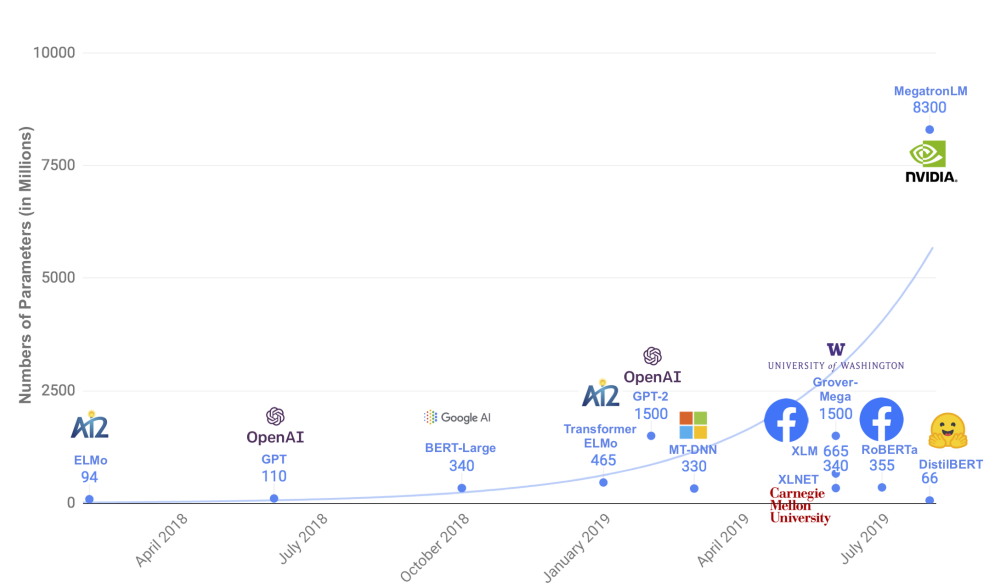
\includegraphics[width = 10cm]{figure/53-distilbert-motivation}\\ 
		\citebutton{Source: Sanh et al., 2019}{https://arxiv.org/pdf/1910.01108.pdf}
	\end{figure}
	
\end{frame}

% ------------------------------------------------------------------------------

\begin{frame}{Model distillation}

\vfill

\textbf{Types of targets} 

\begin{itemize}
	\item ``\textit{Hard}`` Targets $$[0, 0, 0, 1, 0]$$ \vspace{-.5cm}
		\begin{itemize}
			\item Present when learning from labeled data
			\item Ordinary way of training models
		\end{itemize}
	\item Knowledge transfer possible via ``\textit{soft}`` targets from original model
	\item Possible ``\textit{soft}`` targets
		\begin{itemize}
			\item Logits + L2 loss \citebutton{Bucila et al., 2006}{http://www.niculescu-mizil.org/papers/rtpp364-bucila.rev2.pdf}
			\item Softmax scores
			\item Temperature $T$ in the softmax \citebutton{Hinton et al., 2015}{https://arxiv.org/abs/1503.02531}
						$$q_i = \frac{\exp(z_i/T)}{\sum_j \exp(z_j/T)}$$
		\end{itemize}
\end{itemize}

\vfill

\end{frame}

% ------------------------------------------------------------------------------

\begin{frame}{Model distillation}

\vfill

\textbf{Temperature:}\\$$q_i = \frac{\exp(z_i/T)}{\sum_j \exp(z_j/T)}$$

\begin{itemize}
	\item \textit{Why?} Produce a softer probability distribution over classes
	\item $z_i$/$z_j$ are the raw logits
	\item Parameter $T$ controls to smoothness of the distribution
		\begin{itemize}
			\item Higher $T$: ``softer`` distribution
			\item Lower $T$: more pronounced distribution
		\end{itemize}
	\item \textit{Distillation phase}: Apply same temperature to teacher and student
	\item \textit{Inference}: Set $T = 1$ to recover standard softmax						
\end{itemize}

\vfill

\end{frame}

% ------------------------------------------------------------------------------

\begin{frame}{Model distillation}

\vfill

\textbf{Intuition}

\begin{itemize}
	\item Train the student to \textit{mimick} the teacher's behaviour
	\item \ques Advantage of the soft targets:
	\item[] $\to$ No need to know the true labels of the training instances
	\item[] $\to$ More fine-grained information about the teacher's behaviour 
	\item When true labels are known:\\
				Weighted average of two different objective functions possible\\
	\item[] $\to$ On soft targets (\textit{Be close to the teacher}) and 
	\item[] $\to$ on hard targets (\textit{be close to the ``ground truth``})
\end{itemize}

\vfill

\end{frame}

% ------------------------------------------------------------------------------

\begin{frame}{distilbert}

\vfill

\textbf{Characteristics of the student architecture:}

\begin{itemize}
	\item Half the number of layers compared to BERT$^1$ (6 instead of 12)
	\item Remove segment embeddings$^2$ (required for NSP objective)
 	\item Half of the size of BERT, but retains up to 97\% of the performance on GLUE
	\item Initialize from BERT (taking one out of two hidden layers)
	\item Same pre-training data as BERT (Wiki + BooksCorpus)
\end{itemize}

\vfill

{\footnotesize $^1$Rationale for "only" reducing the number of layers:\\
Larger influence on the computation efficiency compared to e.g. hidden size dimension\\
$^2$ Sanh et al. call them ``token-type embeddings`` in their paper}

\end{frame}

% ------------------------------------------------------------------------------

\begin{frame}{distilbert}

\vfill

\textbf{Combination of three different loss functions:}

\begin{itemize}
	\item \textit{Soft targets:}\\Distillation loss $L_{ce} = \sum_i t_i \cdot \log(s_i)$
	\item \textit{Hard targets:}\\Masked language modeling loss $L_{mlm}$ (cf. BERT)
	\item \textit{Alignment:}\\Cosine-Embedding-Loss $L_{cos} = 1 - \frac{\vec w^{(i)T}\vec w^{(j)}}{\lVert \vec w^{(i)} \rVert_2 \cdot \lVert \vec w^{(j)}\lVert_2}$\\
				(\textit{Rationale:} Keep DistilBERT's embeddings close to BERT's)
\end{itemize}

\vspace{.3cm}

\textbf{Adopt improvement from RoBERTa:}

\begin{itemize}
	\item Stop using the NSP loss (hence removed segment embeddings)
	\item Dynamic masking for MLM
	\item Train with large batches
\end{itemize}

\vfill

\end{frame}

% ------------------------------------------------------------------------------

\begin{frame}{distilbert}

\vfill

	\textbf{Performance differences to BERT:}

	\begin{figure}
		\centering
		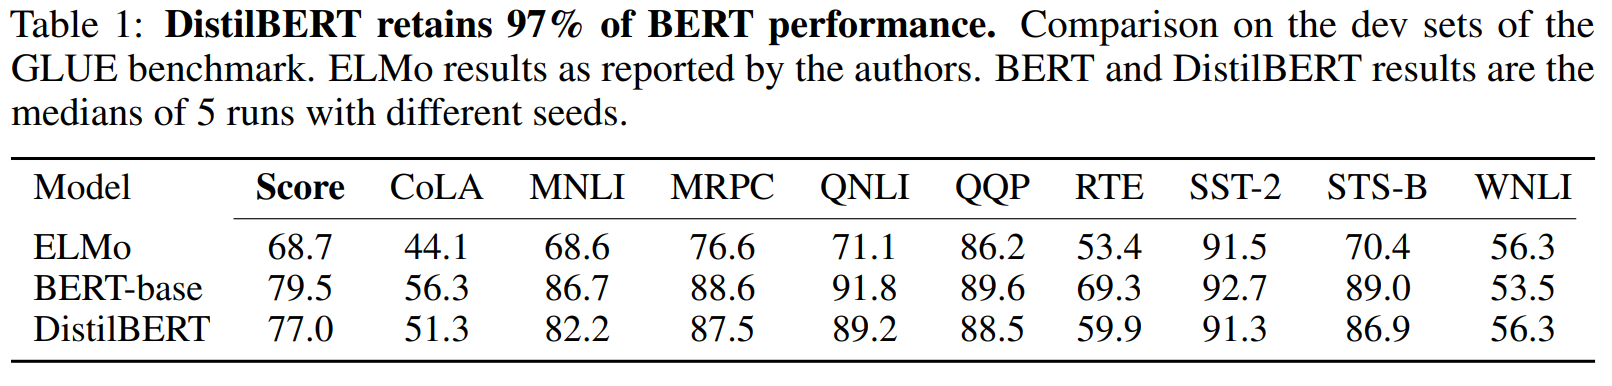
\includegraphics[width = 11cm]{figure/53-distilbert-vs-sota.png}\\ 
		\citebutton{Source: Sanh et al., 2019}{https://arxiv.org/pdf/1910.01108.pdf}
	\end{figure}


\textbf{Takeaways:}

\begin{itemize}
	\item Largest performance on textual entailment task (RTE)
	\item Even better reported performance on Winograd schemas (WNLI)
	\item \textit{Overall:} Very consistent performance a little worse than BERT
\end{itemize}

\vfill

\end{frame}

% ------------------------------------------------------------------------------

\begin{frame}{distilbert}

\vfill

	\textbf{Ablation study regarding the loss:}

	\begin{figure}
		\centering
		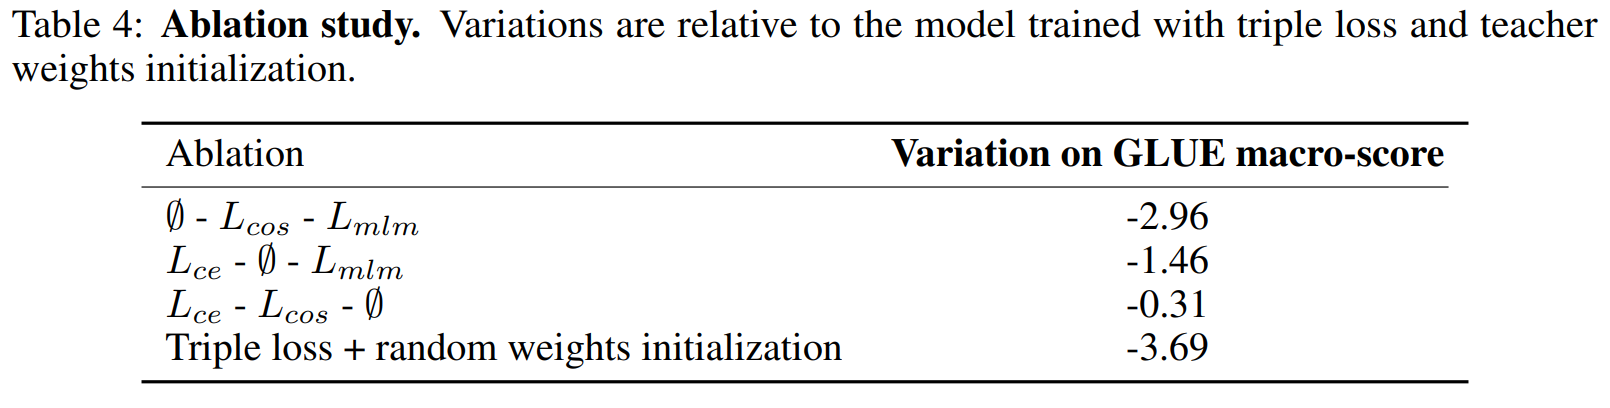
\includegraphics[width = 11cm]{figure/53-distilbert-ablation.png}\\ 
		\citebutton{Source: Sanh et al., 2019}{https://arxiv.org/pdf/1910.01108.pdf}
	\end{figure}

\textbf{Takeaways:}

\begin{itemize}
	\item Start training from BERT's weights is crucial
	\item Removing MLM loss has little impact\\
	\item[] $\to$ Signal in the soft targets sufficiently strong
	\item Notable contribution of the cosine embedding loss
\end{itemize}

\vfill
	
\end{frame}

% ------------------------------------------------------------------------------

\begin{frame}{distilbert}

\vfill

\textbf{Size and speed:}

	\begin{figure}
		\centering
		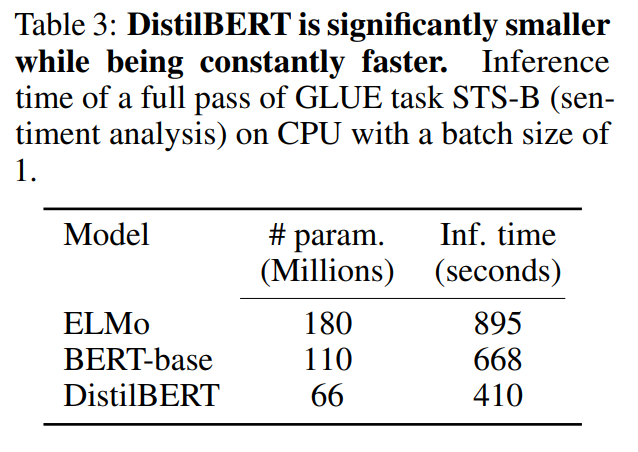
\includegraphics[width = 6.5cm]{figure/53-distilbert-size-speed.png}\\ 
		\citebutton{Source: Sanh et al., 2019}{https://arxiv.org/pdf/1910.01108.pdf}
	\end{figure}

\vfill
	
\end{frame}

% ------------------------------------------------------------------------------

\begin{frame}{related approaches (1)}

\vfill

\textbf{Quantization:}

\begin{itemize}
	\item \textit{In General:} Mathematical procedure of converting a number from a continuous scale to a discrete scale
	\item \textit{In Machine Learning (usually):} Convert a number from high precision (float16/float32) to a lower precision (float8/int8) 
	\item For models with billions of parameters, this can save enormous amount of memory
	\item Given that model sizes (at the moment) grow faster than GPU memory, this can be crucial for even making \textit{inference} of large models feasible
	\item \textit{Trade-Off:} Memory savings vs. model quality
\end{itemize}

\vfill
	
\end{frame}

% ------------------------------------------------------------------------------

\begin{frame}{related approaches (2)}

\vfill

\textbf{Pruning:}

\begin{itemize}
	\item Remove (``\textit{prune}``) certain parts of the model according to some score measuring the importance of that part for performance 
	\item Common importance score (in NLP):\\Sensitivity of the loss wrt the values of the neurons \citebutton{Yang et al., 2022}{https://arxiv.org/abs/2203.15996}
							$$\mathrm{IS}(\bm\Theta) = \mathbb{E}_{x\sim X}\left\lvert \frac{\partial \mathcal{L}(x)}{\partial\bm\Theta}\bm\Theta \right\rvert$$
	\item Common choices for $\bm\Theta$ (in Transformers):
			\begin{itemize}
				\item Output of an attention head
				\item An intermediate neuron in the FFN layer
			\end{itemize}
\end{itemize}

\vfill
	
\end{frame}

% ------------------------------------------------------------------------------

\begin{frame}{related approaches (2)}

\vfill

\textbf{Self-supervised Pruning} \citebutton{Yang et al., 2022}{https://arxiv.org/abs/2203.15996}

\begin{itemize}
	\item Substitute $\mathcal{L}$ by
							$$\mathcal{L}_{\mathrm{KL}}(x)=\mathrm{KL}(\mathrm{stopgrad}(q(x))||p(x)),$$
	\item where
			\begin{itemize}
				\item $q(x)$ is the original model prediction distribution,
				\item $p(x)$ is the to-be-pruned model prediction distribution,
				\item and \texttt{stopgrad} is used to stop back-propagating gradients
			\end{itemize}
\end{itemize}

\vfill
	
\end{frame}

% ------------------------------------------------------------------------------

\begin{frame}{summary}

\vfill

\begin{itemize}
	\item Model compression/distillation against growing model sizes
	\item DistilBERT as a powerful, small alternative to BERT
	\item Other approaches (pruning) that allow for a more targeted ``deactivation`` of individual heads (and might thus also improve interpretability)
	\item Quantization as an approach to \textit{significantly} reduce the memory requirements of large models
\end{itemize}

\vfill
	
\end{frame}

% ------------------------------------------------------------------------------

\endlecture
\end{document}
